% vim: set tw=78 tabstop=4 shiftwidth=4 aw ai:
\documentclass{beamer}

\usepackage[utf8x]{inputenc}		% diacritice
\usepackage[romanian]{babel}
\usepackage{color}			% highlight
\usepackage{alltt}			% highlight

% highlight; comment this out in case you don't input code source files
%\usepackage{code/highlight}		% highlight

\usepackage{hyperref}			% folosiți \url{http://...}
					% sau \href{http://...}{Nume Link}
\usepackage{verbatim}

\mode<presentation>
{
%\usetheme{Madrid} 
%\usetheme{default}
%\usetheme{AnnArbor}
%\usetheme{Antibes}
%\usetheme{Bergen}
%\usetheme{Berkeley}
\usetheme{Berlin}
%\usetheme{Boadilla}
%\usetheme{CambridgeUS}
%\usetheme{Copenhagen}
%\usetheme{Darmstadt}
%\usetheme{Dresden}
%\usetheme{Frankfurt}
%\usetheme{Goettingen}
%\usetheme{Hannover} -nu
%\usetheme{Ilmenau}
%\usetheme{JuanLesPins}
%\usetheme{Luebeck} -poate
%\usetheme{Madrid}
%\usetheme{Malmoe}
%\usetheme{Marburg}
%\usetheme{Montpellier}
%\usetheme{PaloAlto}
%\usetheme{Pittsburgh}
%\usetheme{Rochester}
%\usetheme{Singapore}
%\usetheme{Szeged}
%\usetheme{Warsaw}

% As well as themes, the Beamer class has a number of color themes
% for any slide theme. Uncomment each of these in turn to see how it
% changes the colors of your current slide theme.

%\usecolortheme{albatross}
%\usecolortheme{beaver}
%\usecolortheme{beetle}
%\usecolortheme{crane}
\usecolortheme{dolphin}
%\usecolortheme{dove}
%\usecolortheme{fly} -NU
%\usecolortheme{lily}
%\usecolortheme{orchid}
%\usecolortheme{rose}
%\usecolortheme{seagull}
%\usecolortheme{seahorse}
%\usecolortheme{whale}
%\usecolortheme{wolverine}

}

% Încărcăm simbolurilor Unicode românești în titlu și primele pagini
\PreloadUnicodePage{200}

% Arătăm numărul frame-ului
\newcommand{\frameofframes}{/}
\newcommand{\setframeofframes}[1]{\renewcommand{\frameofframes}{#1}}

\setframeofframes{of}
\makeatletter
\setbeamertemplate{footline}
  {%
    \begin{beamercolorbox}[colsep=1.5pt]{upper separation line foot}
    \end{beamercolorbox}
    \begin{beamercolorbox}[ht=2.5ex,dp=1.125ex,%
      leftskip=.3cm,rightskip=.3cm plus1fil]{author in head/foot}%
      \leavevmode{\usebeamerfont{author in head/foot}\insertshortauthor}%
      \hfill%
      {\usebeamerfont{institute in head/foot}\usebeamercolor[fg]{institute in head/foot}\insertshortinstitute}%
    \end{beamercolorbox}%
    \begin{beamercolorbox}[ht=2.5ex,dp=1.125ex,%
      leftskip=.3cm,rightskip=.3cm plus1fil]{title in head/foot}%
      {\usebeamerfont{title in head/foot}\insertshorttitle}%
      \hfill%
      {\usebeamerfont{frame number}\usebeamercolor[fg]{frame number}\insertframenumber~\frameofframes~\inserttotalframenumber}
    \end{beamercolorbox}%
    \begin{beamercolorbox}[colsep=1.5pt]{lower separation line foot}
    \end{beamercolorbox}
  }
\makeatother

\setbeamertemplate{navigation symbols}{}%remove navigation symbols

\title[Analiza traficului și profile utilizatori în rețele virtualizate pentru decizii de caching]{Analiza traficului și profile utilizatori în rețele virtualizate pentru decizii de QoS }
\subtitle{Sesiunea de licență -- iulie 2015}
\institute[Universitatea POLITEHNICA București]{Facultatea de Automatică și Calculatoare,\\
	Universitatea POLITEHNICA București}
\author[Cristina Opricean\u a]{Cristina Georgiana Opricean\u a\\
	Coordonator: R\u azvan Deaconescu}
\date{9 iulie 2015}

\begin{document}

% Slide-urile cu mai multe părți sunt marcate cu textul (cont.)
\setbeamertemplate{frametitle continuation}[from second]

% Arătăm numărul frame-ului
%\setbeamertemplate{footline}[frame number]

\frame{\titlepage}



% NB: Secțiunile nu sunt marcate vizual, ci doar apar în cuprins
\section{Context}

% Titlul unui frame se specifică fie în acolade, imediat după \begin{frame},
% fie folosind \frametitle


\begin{frame}{Virtualizarea rețelelor de comunicații}

\begin{enumerate}
\pause
\uncover<1->{\item
Abordare curentă \\~\\ 
 \begin{itemize} [<+->]
 	\item{echipamente dedicate interconectate}
 	\item{routere, switchuri, firewall-uri, IDS/IPS}\\~\\
 \end{itemize} 
}
 \pause
\uncover<2->{\item
Rețele virtualizate \\~\\
	\begin{itemize}	 [<+->]	% Just like normal LaTeX
		\item abstractizare peste infrastructura fizică
		\item mutarea echipamentelor dedicate în software
	\end{itemize}
}
\end{enumerate}

\end{frame}

\begin{frame}{Network Function Virtualization}
	\begin{figure}[H]
	\begin{center}
	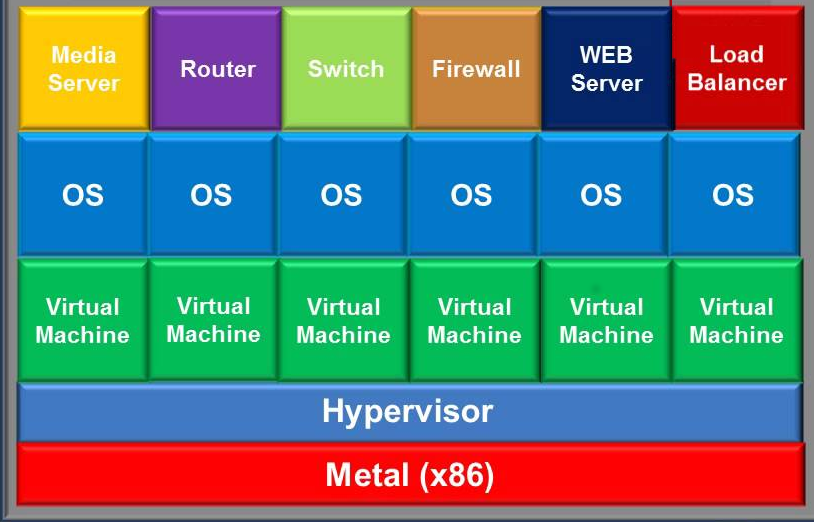
\includegraphics[scale=0.3]{img/nfv.png} 
	
	[1] http://blog.3g4g.co.uk
	\end{center}
	\end{figure}
\end{frame}

\section{Motivație}
\begin{frame}{Motivație}
	\pause
	\begin{itemize} [<+->]
		\item îmbunătățirea experienței utilizatorilor pe Internet
		\item automatizarea procesului de configurare a rețelelor
		\item soluție flexibilă
		\item costuri scăzute prin replicare software
		\item testarea capabilităților NFV
		\item domeniu de reaserch
	\end{itemize}
\end{frame}

\begin{frame}{Ce am realizat?}
\pause
\begin{itemize} [<+->]
	\item {vPersonna, modul NFV cu mai multe capabilități
		\begin{itemize} [<+->]
				\item analiză trafic la nivel II, III în stiva TCP/IP
				\item agregare date
				\item management descentralizat al politicilor de QoS	\\~\\
		\end{itemize}
	}
	
	\item { utlizarea statisticilor pentru decizii
		\begin{itemize} [<+->]
				\item traffic shaping
				\item caching   \\~\\
		\end{itemize}
	}
	\item [] {
		\begin{beamerboxesrounded}[lower=block body,shadow=true]{}
			\texttt{Cui se adresează vPersonna? }
			\begin{itemize}
				\item \texttt{ISP}
			\end{itemize}
		\end{beamerboxesrounded}
	}
	\end{itemize}
	
\end{frame}

\section{Arhitectură și design}

\begin{frame}{Arhitectura aplicației vPersonna}
\pause
	\begin{figure}
		{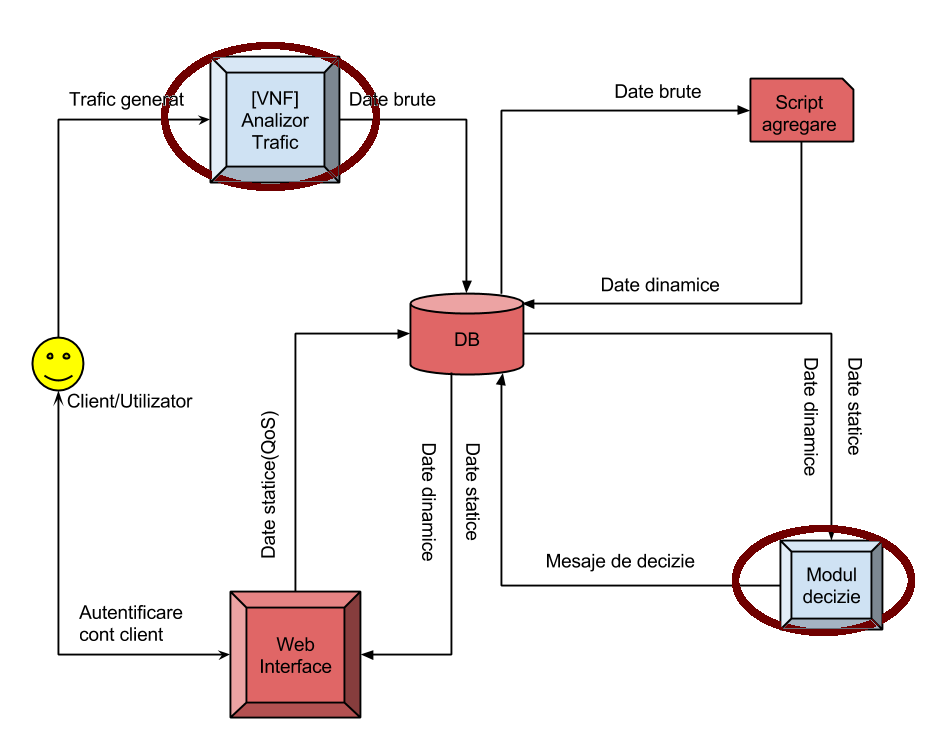
\includegraphics[scale=0.25]{img/vpersonna} }
	\end{figure}
\end{frame}

\section{Implementare}

\begin{frame}{Modulul de achiziție a datelor}
\pause
	\begin{itemize}[<+->]
		\item TCP, agregare în sesiuni
			\begin{itemize}
				\item start sesine: SYN = 1, ACK = 0
				\item final sesiune: FIN = 1
			\end{itemize}
		\item UDP
			\begin{itemize}
				\item inspectare protocol de nivel aplicție
			\end{itemize}
		\item Definirea tipurilor de trafic

		\item [] { \begin{beamerboxesrounded}[lower=block body,shadow=true]{}
				enum type\_of\_service \{HTTP, TORRENT, VoIP, VIDEO, DFLT\};
	
			   \end{beamerboxesrounded}
		}
		\item [] {\begin{block}{Componența unei sesiuni}
				IP Sursă, IP Destinație, Port Sursă, Port Destinație, Tip de Trafic
			   \end{block}
		}
	\end{itemize}	
\end{frame}

\begin{frame}{Recunoașterea tipurilor de trafic}
\pause
	\begin{itemize}[<+->]
		\item pe baza porturilor
		\item HTTP: extragerea campului hostname din header
		\item câmpul MIME din headerul HTTP
		\item VoIP: SIP, H323, ISUP, MGCP, UNISTIM din layerul superior protocolului RTP
		\item TORRENT: porturi specifice
	\end{itemize}
\end{frame}

\begin{frame}{Design software pentru achiziția datelor}
\pause
	\only<1>  {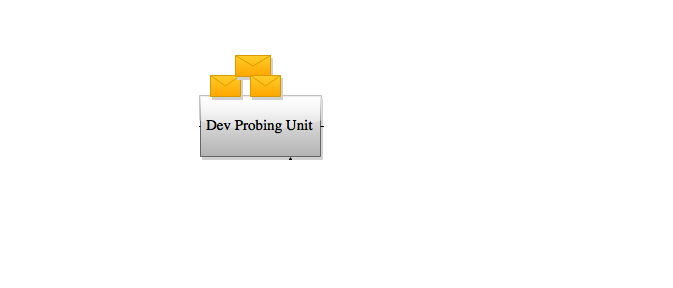
\includegraphics[scale=0.45]{img/1_diag} }
	\only<2>  {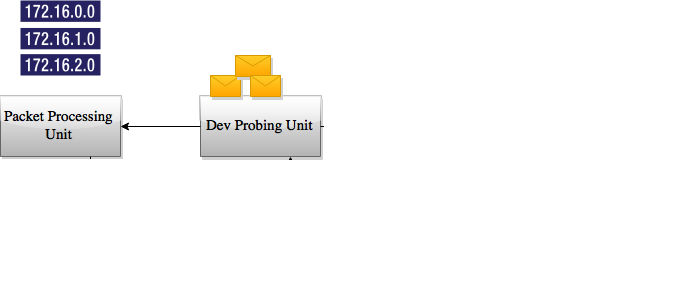
\includegraphics[scale=0.45]{img/2_diag} }
	\only<3>  {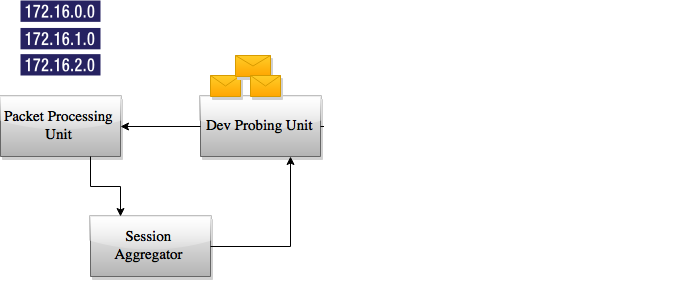
\includegraphics[scale=0.45]{img/3_diag} }
	\only<4>  {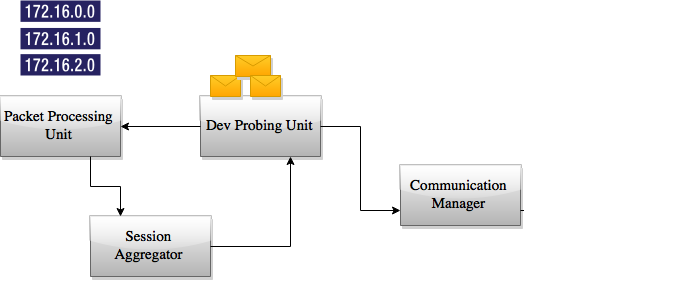
\includegraphics[scale=0.45]{img/4_diag} }
	\only<5>  {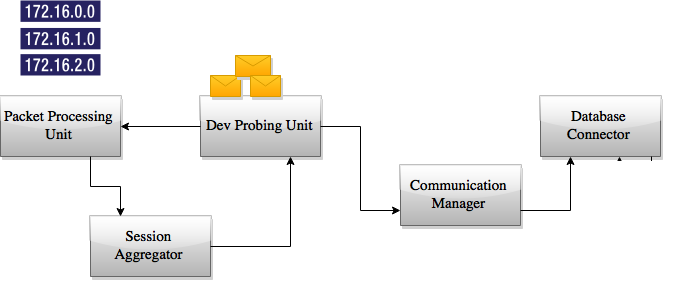
\includegraphics[scale=0.45]{img/5_diag} }
	\only<6>  {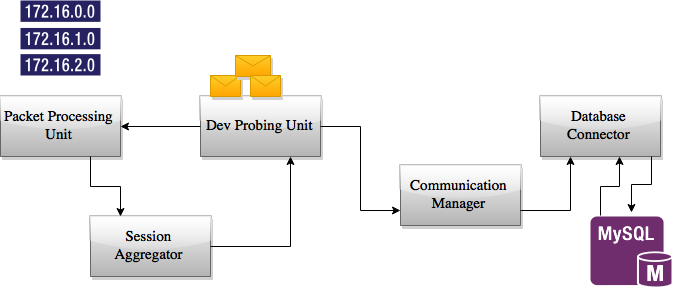
\includegraphics[scale=0.45]{img/6_diag} }
\end{frame}

\begin{frame}{Profilul utilizatorului și interfață}
\pause
	\begin{figure}
        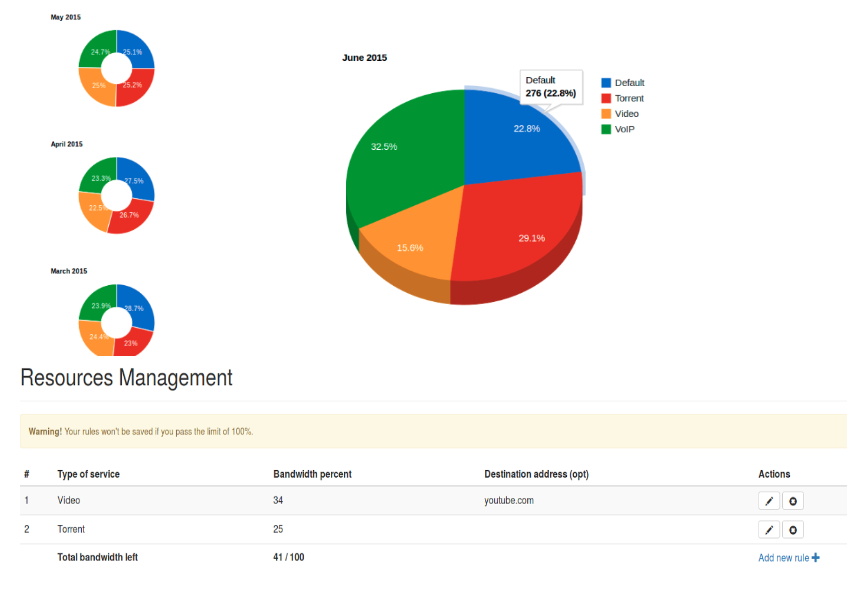
\includegraphics[scale=0.35]{img/iface}
    	\end{figure}
\end{frame}

\begin{frame}{Modulul de decizie}
\pause
	\begin {enumerate} [<+->]
		\item {	Sugestii pentru utilizator
			\begin{itemize} [<+->]
				\item algoritmul K-Clustering
				\item 4 dimensiuni, corespunzătoare tipurilor de trafic
				\item sugestii conform celor mai apropiați vecini
			\end{itemize}
		}
		\item { Caching
			\begin{itemize} [<+->]
				\item heap cu cele mai accesate site-uri
				\item logging al update-urilor
				\item roll-back pentru vizualizare între anumite ore
			\end{itemize}
		}
		\item { proof of concept }
		\item { îmbunătățite pentru ISP }
	\end{enumerate}
\end{frame}

%\begin{frame}{Porțiuni de cod}
%	\input{code/sample}
%\end{frame}
	
\section{Rezultate}

\begin{frame}{Testare și Rezultate(1)}
\pause
	\begin{itemize} [<+->]
	\item Setup Demo
		\begin{itemize} [<+->]
		\item Mai multe mașini virtuale, care simulează clienți
		\item Scapy, POSTGre SQL, Raspberry PI \\~\\
		\end{itemize}
	 \item Concluzii
	 \begin{figure}
        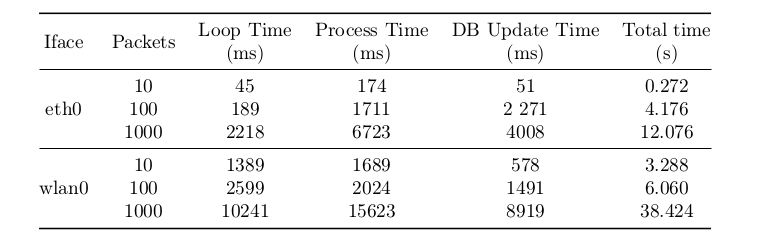
\includegraphics[scale=0.35]{img/tabel}
    	\end{figure}
	 \begin{itemize} [<+->]
	 	\item timp ridicat de looping pe interfețe
	 	\end{itemize}
	\end{itemize}
\end{frame}

\begin{frame}{Testare și Rezultate(2)}
	\begin{itemize}  
		\item Clusterizare simplă
	\end{itemize}
	\begin{figure}
		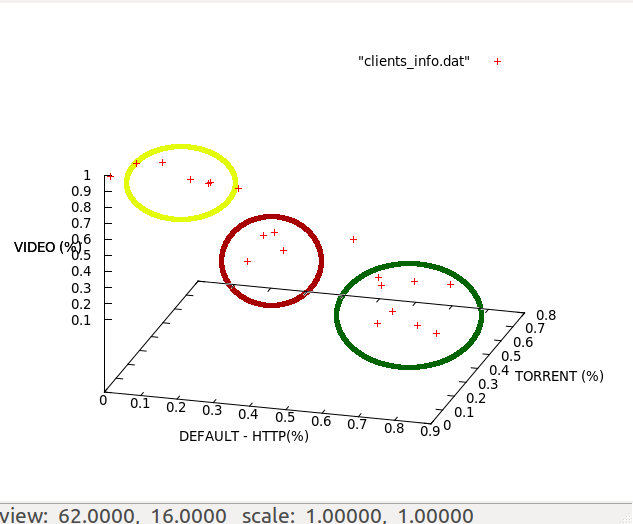
\includegraphics[scale=0.27]{img/cluster_2}
	\end{figure}	
	\begin{itemize} [<+->]
		\item Sugestii utilizator
		\item Autoconfigurare
	\end{itemize}
\end{frame}

\section{\^{I}ntrebări}

\begin{frame}{Concluzii}
\pause
\begin{enumerate} [<+->]
	\item Contribuție
		\begin{itemize} [<+->]
			\item Modulul de achiziție a datelor
			\item Modulul de decizie  \\~\\
		\end{itemize}
	\item Caracteristici
		\begin{itemize} [<+->]
			\item Suport pentru autoconfigurare bandwidth
			\item Flexibilitate și replicare rapidă  \\~\\
		\end{itemize}
	\item Îmbunătățiri ulterioare
		\begin{itemize} [<+->]
			\item Integrare cu framework ClickOS
			\item Creșterea complexității analizei traficului
			\item Sistem de workeri pentru date
			\item Sistem de promoții în profilul utilizatorului
		\end{itemize}		
\end{enumerate}
\end{frame}

\end{document}
